\documentclass{article}
\usepackage[utf8]{inputenc}
\usepackage{caption}
\usepackage[margin=1in]{geometry}
\usepackage{graphicx}
\usepackage{pdfpages}
\usepackage{float}
\pdfminorversion=7

\begin{document}
\begin{titlepage}

\centering
\vspace*{2cm}
{\Huge Code Inspection Report\par}
\vspace{.25cm}
{\LARGE Course Evaluation System\par}
\vspace{1cm}
{\Large Team EVAL\par}
\vspace{.2cm}
{\Large Jovon Craig, Sam Elliott, Robert Judkins, and Stanley Small\par}
\vspace{1cm}
{\Large Client: Dr. Harlan Onsrud\par}
\vspace{1cm}
{\Large March ??, 2019\par}
\vspace{11cm}

University of Maine - Spring 2019 - COS 497

Instructor: Professor Terry Yoo

\end{titlepage}

\newpage

\begin{center}
{
\includegraphics[scale=.2]{images/team_logo.png}} \\ 	\bigskip
{\LARGE Course Evaluation System } \\ \medskip
{\large Code Inspection Report } \\ \medskip
\end{center}

\tableofcontents

\newpage

\section{Introduction}
 
\subsection{Purpose of This Document}



\subsection{References}

Craig, J., Elliott, S., Judkins, R., \& Small, S. 29 October 2018. \textit{System Requirements Specification.}
\vspace{3mm}\newline
Craig, J., Elliott, S., Judkins, R., \& Small, S. 16 November 2018. \textit{System Design Document.}
\vspace{3mm}\newline
Onsrud, H. ``Example Question Selection Form.'' See Appendix D.
\vspace{3mm}\newline
Onsrud, H. ''Report for Professor: Roy Turner'' See Appendix E.

\subsection{Coding and Commenting Conventions}



\subsection{Defect Checklist}



\begin{center}
\captionof{table}{Defect checklist}
\scalebox{.92}{
\begin{tabular}{|p{3cm}|p{8cm}|} 
\hline
\textbf{Category} & \textbf{Statement} \\
\hline
 & \\ 
\hline
 & \\ 
\hline
 & \\ 
\hline
 & \\ 
\hline
 & \\ 
\hline
 & \\ 
\hline
 & \\ 
\hline
 & \\ 
\hline
 & \\ 
\hline
 & \\ 
\hline
 & \\ 
\hline
 & \\ 
\hline
 & \\ 
\hline
 & \\ 
\hline
 & \\ 
\hline
\end{tabular}
}
\end{center}

\section{Code Inspection Process}

\subsection{Description}



\subsection{Impressions of the Process}



\subsection{Inspection Meetings}



\section{Modules Inspected}



\section{Defects}



\begin{center}
\captionof{table}{List of defects found}
\scalebox{.92}{
\begin{tabular}{|p{1.5cm}|p{2.5cm}|p{4cm}|p{3cm}|} 
\hline
\textbf{Number} & \textbf{Module} & \textbf{Description} & \textbf{Category} \\
\hline
 & & & \\ 
\hline
 & & & \\ 
\hline
 & & & \\ 
\hline
 & & & \\ 
\hline
 & & & \\ 
\hline
\end{tabular}
}
\end{center}

\appendix

\newpage
\section{Coding and Commenting Conventions}



\newpage
\section{Agreement Between Customer and Contractor}
This page shows that all members of Team EVAL and the client, Harlan Onsrud, have agreed on all the information in the code inspection report. By signing this document, Team EVAL and Dr. Onsrud approve the coding conventions used, the information about the inspection process, and the descriptions of the defects and inspected modules.

The team will follow a process in the case that the document is changed after we sign it. First, the team will write a rough draft of the changes to be made to the document. Second, all team members and Harlan Onsrud will sign the document agreeing to the changes. Finally, the team will make the changes to the final copy of the document.

\vspace{.7in}
\noindent
\begin{tabular}{ p{5cm} p{5cm} p{5cm} } 
\textbf{\textit{Name}} & \textbf{\textit{Signature}} & \textbf{\textit{Date}} \\[.5cm]
\textbf{Jovon Craig} & $\rule{5cm}{.1mm}$ & $\rule{5cm}{.1mm}$\\[.5cm]
\textbf{Sam Elliott} & $\rule{5cm}{.1mm}$ & $\rule{5cm}{.1mm}$\\[.5cm]
\textbf{Robert Judkins} & $\rule{5cm}{.1mm}$ & $\rule{5cm}{.1mm}$\\[.5cm]
\textbf{Stanley Small} & $\rule{5cm}{.1mm}$ & $\rule{5cm}{.1mm}$\\[.5cm]
\textbf{Harlan Onsrud} & $\rule{5cm}{.1mm}$ & $\rule{5cm}{.1mm}$\\[.5cm]
Customer Comments: & \multicolumn{2}{ l }{ $\rule{10.45cm}{.1mm}$ }\\[.5cm]
\multicolumn{3}{ l }{ $\rule{15.9cm}{.1mm}$ }\\[.5cm]
\end{tabular}

\newpage
\section{Team Review Sign-off}

This page shows that all members of Team EVAL have reviewed the code inspection report and agreed on its content. By signing this document, the team members agree that all information about Team EVAL's code inspections is accurate, and there is nothing in the document that is a source of contention.

\vspace{.7in}
\noindent
\begin{tabular}{ p{5cm} p{5cm} p{5cm} } 
\textbf{\textit{Name}} & \textbf{\textit{Signature}} & \textbf{\textit{Date}} \\[.5cm]
\textbf{Jovon Craig} & $\rule{5cm}{.1mm}$ & $\rule{5cm}{.1mm}$\\[.5cm]
Comments: & \multicolumn{2}{ l }{ $\rule{10.45cm}{.1mm}$ }\\[.5cm]
\multicolumn{3}{ l }{ $\rule{15.9cm}{.1mm}$ }\\[.5cm]
\textbf{Sam Elliott} & $\rule{5cm}{.1mm}$ & $\rule{5cm}{.1mm}$\\[.5cm]
Comments: & \multicolumn{2}{ l }{ $\rule{10.45cm}{.1mm}$ }\\[.5cm]
\multicolumn{3}{ l }{ $\rule{15.9cm}{.1mm}$ }\\[.5cm]
\textbf{Robert Judkins} & $\rule{5cm}{.1mm}$ & $\rule{5cm}{.1mm}$\\[.5cm]
Comments: & \multicolumn{2}{ l }{ $\rule{10.45cm}{.1mm}$ }\\[.5cm]
\multicolumn{3}{ l }{ $\rule{15.9cm}{.1mm}$ }\\[.5cm]
\textbf{Stanley Small} & $\rule{5cm}{.1mm}$ & $\rule{5cm}{.1mm}$\\[.5cm]
Comments: & \multicolumn{2}{ l }{ $\rule{10.45cm}{.1mm}$ }\\[.5cm]
\multicolumn{3}{ l }{ $\rule{15.9cm}{.1mm}$ }\\[.5cm]
\end{tabular}


\newpage
\section{Document Contributions}

Stanley Small ??. Stan contributed approximately ?? percent of the document.

Jovon Craig ??. Jovon contributed about ?? percent of the document.

Sam Elliott ??. Sam contributed about ?? percent of the document.

Robert Judkins ??. Robert contributed about ?? percent of the document.

\newpage

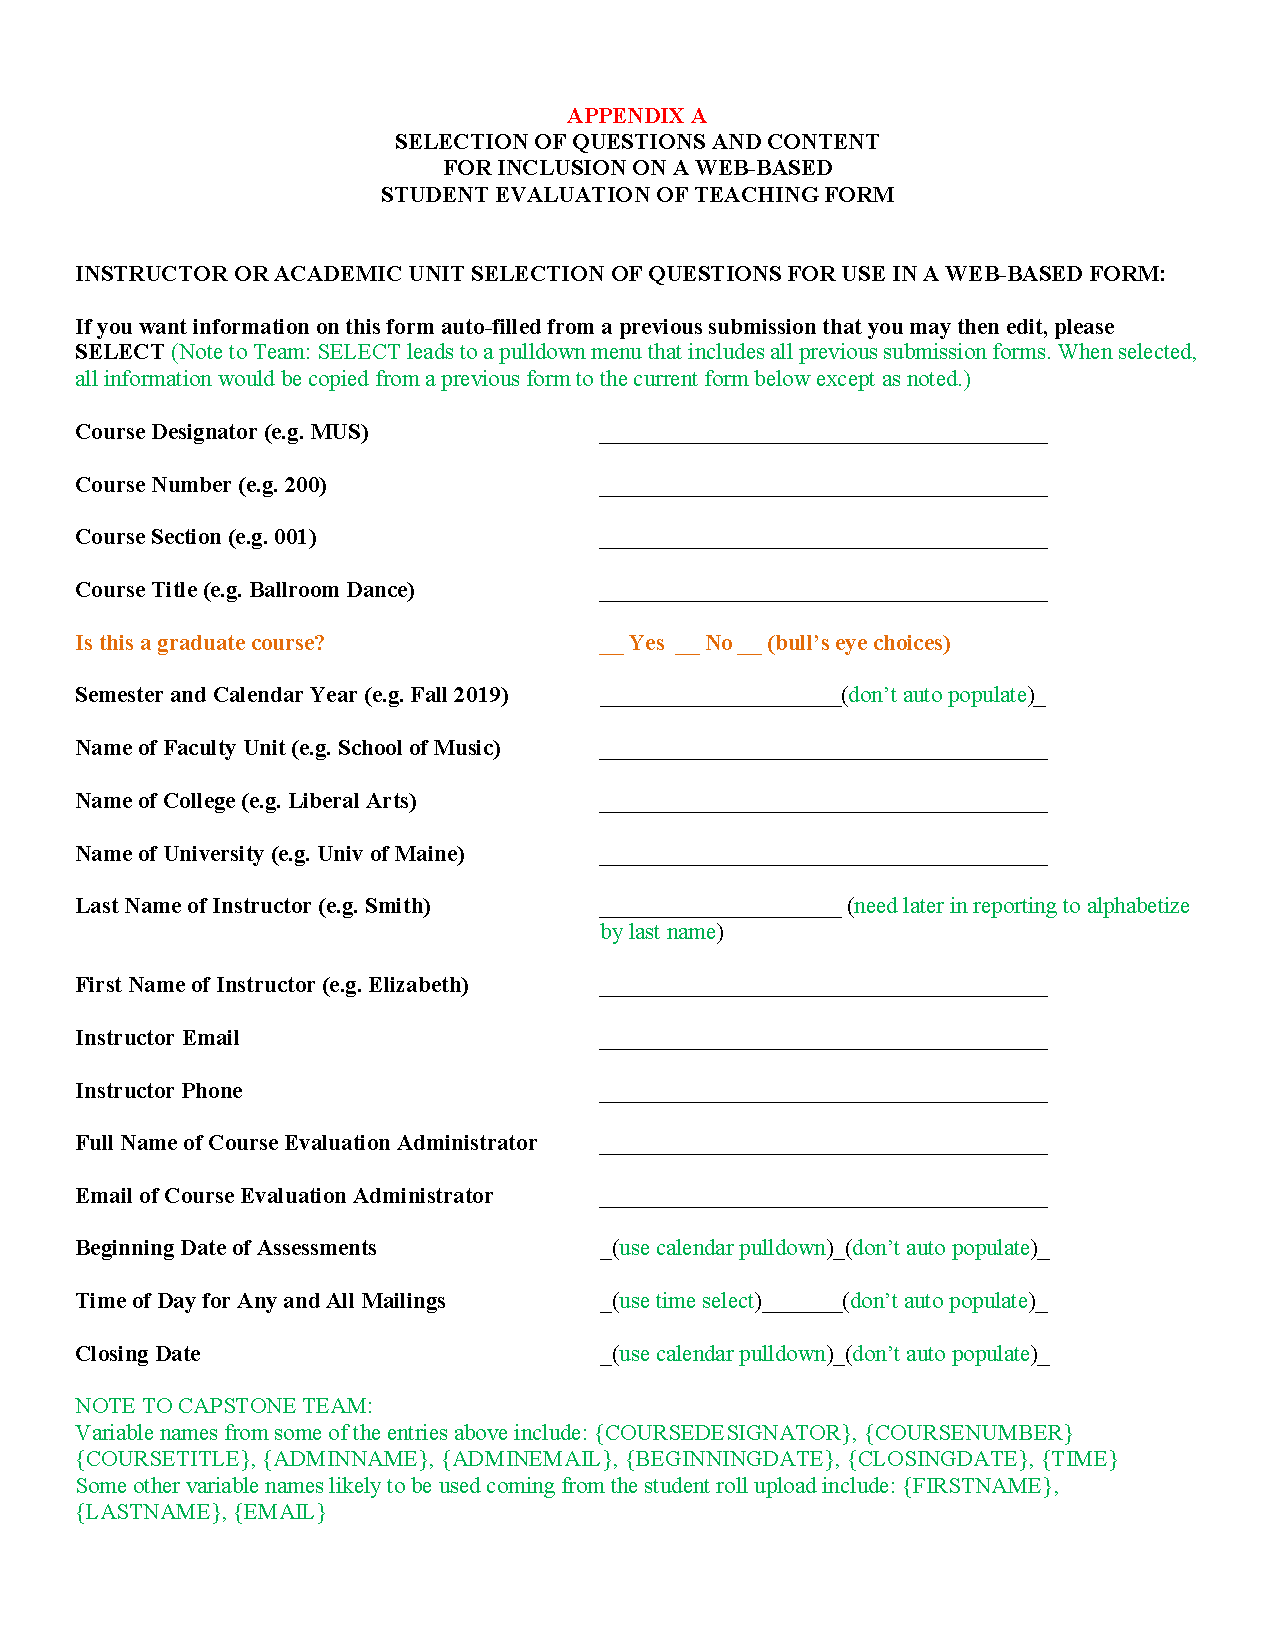
\includepdf[scale=0.85,pages=1,pagecommand=\section{Example Question Selection Form}]{images/question_appendix.pdf}
\includepdf[scale=0.85,pages=2-]{images/question_appendix.pdf}

\newpage

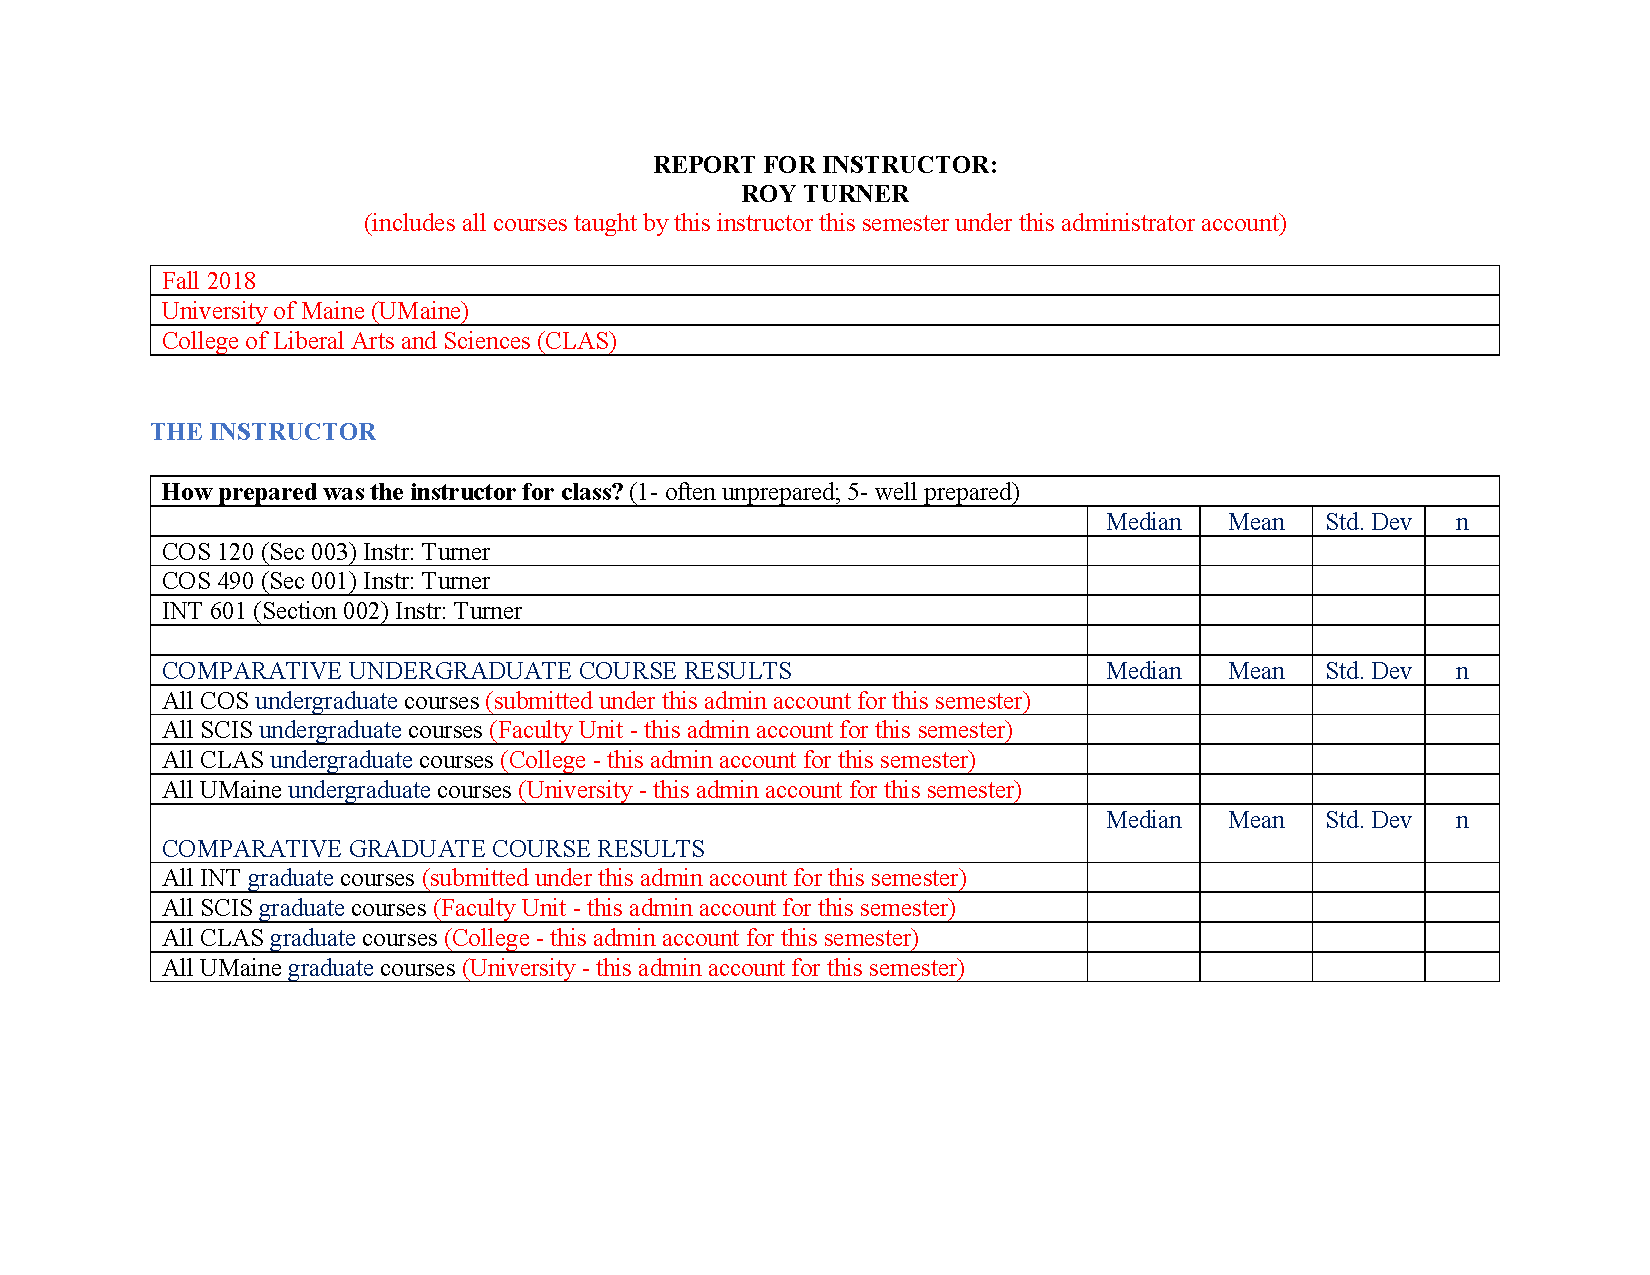
\includepdf[scale=0.92,pages=1,pagecommand=\section{Example Results Display}]{images/results_appendix.pdf}
\includepdf[scale=0.92,pages=2-]{images/results_appendix.pdf}
\end{document}
